Figure \ref{fig:siso-subband} illustrates the R-E region against subband $N = 1,2,4,8,16$ for superposed waveform and no power waveform in FF and FS channels respectively.

\begin{figure}[ht]
  \centering
  \subfigure[FF: Superposed waveform]{
    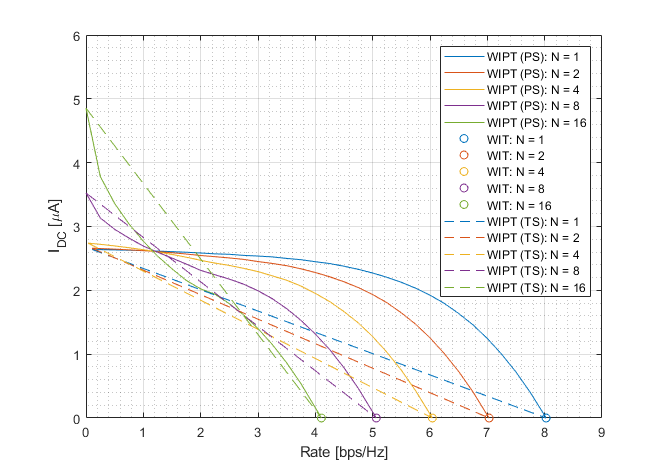
\includegraphics[width=0.48\textwidth]{siso_re_ff_subband_superposed_waveform}\label{fig:subband-ff-superposed}}
  \subfigure[FF: No power waveform]{
    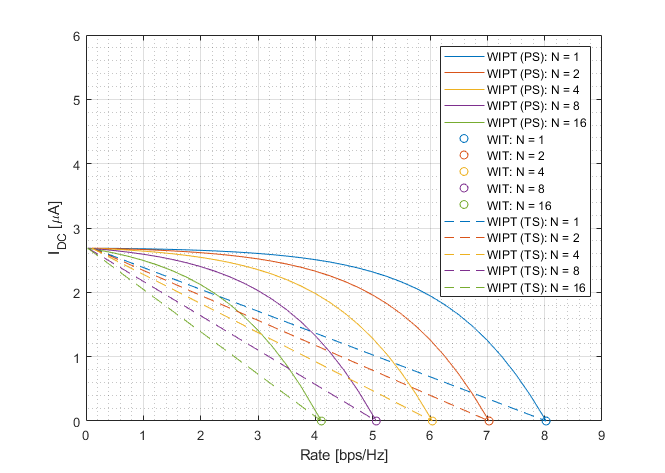
\includegraphics[width=0.48\textwidth]{siso_re_ff_subband_no_power_waveform}\label{fig:subband-ff-no-power}}
  \quad
  \subfigure[FS: Superposed waveform]{
    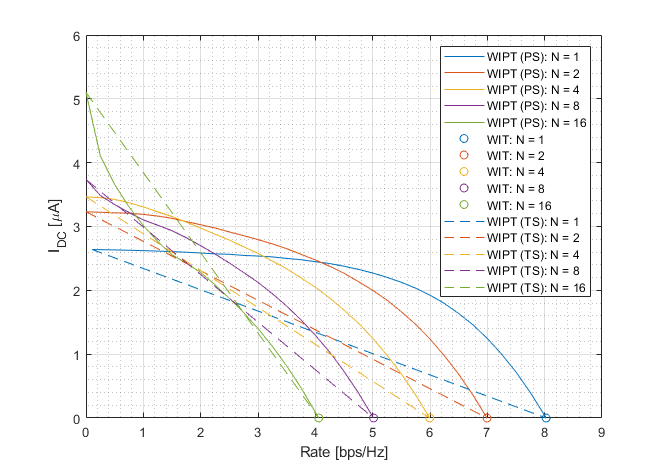
\includegraphics[width=0.48\textwidth]{siso_re_fs_subband_superposed_waveform}\label{fig:subband-fs-superposed}}
  \subfigure[FS: No power waveform]{
    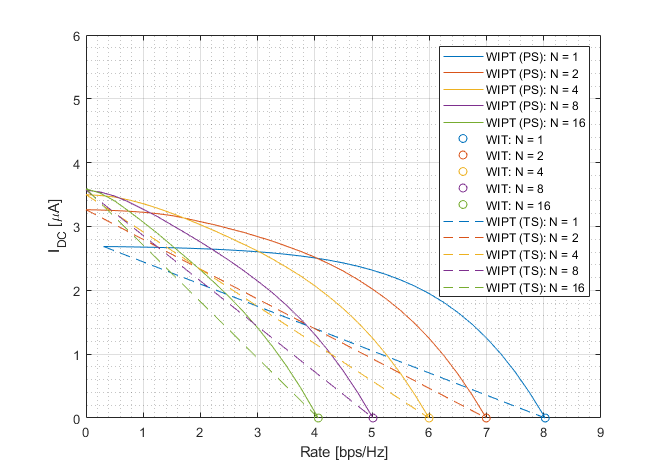
\includegraphics[width=0.48\textwidth]{siso_re_fs_subband_no_power_waveform}\label{fig:subband-fs-no-power}}
  \caption{R-E region vs $N$ for FF and FS channels}\label{fig:siso-subband}
\end{figure}

It can be observed that the introduction of multisine power waveform boosts the harvested energy for $N > 4$ where the superposed waveform outperforms the modulated signal for WIPT. In contrast, the R-E performance of both signals are very close for $N \leqslant 4$ and the modulated waveform is preferred with lower complexity. The reason is that the fourth order terms of power and information waveforms \ref{eqn:power_waveform_fourth_order} and \ref{eqn:information_waveform_fourth_order} have different contribution to the harvested DC current. Despite both posynomials consist of monomials of similar magnitude (${\prod\nolimits_{j = 0}^3 {{s_{P,{n_j},{m_j}}}{A_{{n_j},{m_j}}}} }$ and $\prod\nolimits_{j = 0,2} {{s_{I,{n_0},{m_j}}}{A_{{n_0},{m_j}}}} \prod\nolimits_{j = 1,3} {{s_{I,{n_1},{m_j}}}{A_{{n_1},{m_j}}}} $ ), the power posynomial contains $(2{N^3} + N)/3$ monomials but the information posynomial only holds ${N^2}$ monomials. Therefore, the benefit of multisine power waveform on the harvested power is amplified with a large $N$. Although it seems that a very large $N$ can further increases the output DC current, this is not the case as each subband receives less portion and the amplitude of monomials decreases accordingly.

A contrast of R-E plots on FF and FS channels also indicates the benefit of frequency selectivity on the harvested power. The gain is particularly obvious in the low-rate region, where all the power is allocated to the subband with strongest amplitude. Consider the FS channel instance denoted by Figure \ref{fig:siso-fs}. Some edge frequencies enjoy a larger gain than the center frequency, whose advantage is exploited when more subbands are used in WIPT. In comparison, the small amplitude at the center frequency accounts for the lower output DC current when $N = 1$ (indicated by the blue curves in \ref{fig:subband-fs-superposed} and \ref{fig:subband-fs-superposed}). The result is inline with the scaling laws proposed in \cite{Clerckx2018}.

Another finding is that without power waveform, the R-E region appears convex such that PS dominates for all $N$. On the other hand, the R-E region with the superposed waveform by PS is convex for $N = 2,4$ but concave-convex for $N = 8,16$. Therefore, the optimal strategy is PS for small $N$, TS for large $N$, and a combination of PS and TS for medium $N$. As illustrated in Figure \ref{fig:siso-subband-optimal}, the best curve for medium $N$ consists of two parts. The straight part is achieved by TS between WPT (multisine only and $\rho  = 1$) that corresponds to the leftmost point and WIPT (superposed waveform with $0 < \rho  < 1$) that corresponds to the tangent point, while the convex part is the contribution of WIPT only. The characteristics of the optimal R-E region comes from the rectifier nonlinearity.

\begin{figure}[ht]
  \centering
  \subfigure[Optimal strategy for $N = 8$]{
    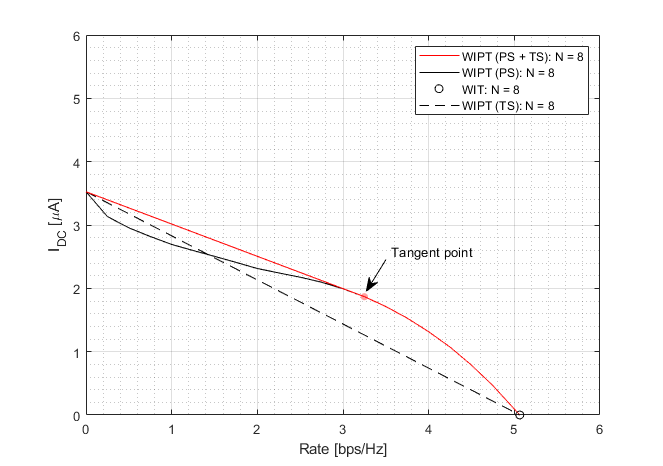
\includegraphics[width=0.48\textwidth]{siso_re_ff_subband_8_optimal}\label{fig:subband-8-optimal}}
  \subfigure[Optimal strategy for $N = 16$]{
    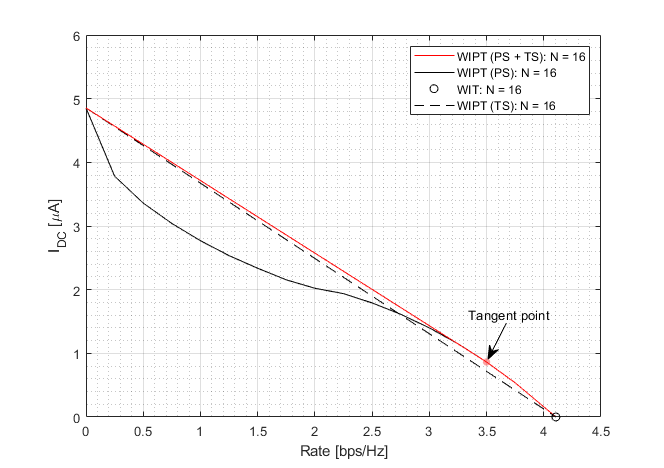
\includegraphics[width=0.48\textwidth]{siso_re_ff_subband_16_optimal}\label{fig:subband-16-optimal}}
  \caption{Optimal R-E region for FF channel with medium $N$}\label{fig:siso-subband-optimal}
\end{figure}

One main problem of the results is that the leftmost point of some curves did not start from the y-axis. This is because although a zero rate constraint is employed in WIPT, a candidate solution may achieve a nonzero rate. However, if the current gain of the next iteration is smaller than the threshold $\varepsilon$, the algorithm terminates and outputs the existing R-E pair. This phenomenon occurs primarily for small $N$ that produces a lower harvested current (hence smaller gain in each iteration) and low-rate region where the output DC current almost saturated. It can be fixed either by reducing threshold $\varepsilon$ or developing an individual function for WPT.

